\section{Formalizing the Field of Work} % (fold)
\label{sec:formalizaing_the_field_of_work}
In general, the field of work in a collaborative activity can be defined as a domain model that includes three related sub-models $FoW=\{ER, LS, DEP\}$: the model of basic entities and their relations $ER$, the set of all actors' local scopes $LS$, and the set of dependencies among activities $DEP$. $ER$ provides the basic vocabulary for defining local scopes $LS$ and dependencies $DEP$. We elaborate on the three components in the rest of this section. 

\subsection{Entities and relations} % (fold)
\label{sub:entities_relations}
\subsubsection{Entities} % (fold)
\label{ssub:entities}
Following the conceptualization of the field of work in Section \ref{sub:the_field_of_work}, 
we define three basic entities that are the basic building blocks in a collaborative activity:
\begin{enumerate}
    \item \textbf{Actors} are defined as human actors participated in a collaborative activity, capable of making decisions and performing actions. $AR=\{ar_1, ar_2, ..., ar_n\}$ is the set of all the actors in a collaborative activity.
    \item \textbf{Resources} are anything that can be used in the transformation process of an activity, including both material resource and resources for thinking. We use $RES=\{res_1, res_2, ..., res_n\}$ to denote the set of resources used in a collaborative activity.
	\item \textbf{Actions} include all the actions that have been performed, is under execution, or will be performed in a collaborative activity. $ACT=\{a_1, a_2, ..., a_n\}$ denotes the set of actions. 
\end{enumerate}

We presume all the basic entities fall into types. Each \emph{action type} represents a class of actions that can be performed by executing a set of subsidiary tasks, commonly called a \emph{recipe}. For example, an actor might rent a car by walking to the rental car center, selecting the car, paying the money, and so forth. Each \emph{resource type} represents a class of resource objects that share the same list of properties and behaviors. For example, every car at the rental car center has a make, model, rental price, etc. Each \emph{actor type} represents a role that abstracts the behaviors of a social actor within some specialized context or domain of endeavor \cite{Bresciani2004}. Its characteristics are easily transferable to other social actors. For example, every actor at the rental car center in the role of `receptionist' can help the customer to rent a car.

We follow Hunsberger and Ortiz \cite{Hunsberger} to use the $@$ constructor to make the distinction between types and instances of entities in the formalization. Each type expression is defined as a unique keyword (e.g. $AType$), then each instance is in the form of the type keyword followed by a set of arguments necessary to identify it (e.g. $AType@arg_1(val_1)@arg_2(val_2)...@arg_n(val_n)$). For example, $drive$ can be an action type and an instance could be $drive@car(car_3)@from(loc_1)@to(loc_2)$ that specifies an instance of driving $car_3$ from location $loc_1$ to $loc_2$. $receptionist@name(Mike)$ is an actor named $Mike$ in the role of $receptionist$. To simplify the expression, we may sometimes use a type keyword followed by a subscript to define an instance. For example, $receptionist_1$ can be used to define an instance of $receptionist$.

% subsubsection entities (end)
\subsubsection{Relations} % (fold)
\label{ssub:relations}
The relations between these entities can be defined using predicate symbols. For example, predicate symbol $Located_in$ can be used to indicate the spatial relation of one entity is inside the second entity. The fact that actor $ar_1$ is in the office $room_3$ can be expressed as $Located_in(ar_1, room_3)$. The list of predicate symbols and their meanings are usually domain dependent. However, here we are more interested in defining a subset of relations between these entities that reflect the common characteristics of activity structure, and are used later to define the local scopes $LS$ and dependencies $DEP$.

\paragraph*{Actor's intention towards action} % (fold)
\label{par:relations_between_action_and_agent}
We follow the SharedPlans theory \cite{grosz1996collaborative} to define three types of intention predicates, $Pot.Int$, $Int.Th$, and $Int.To$, to represent the \emph{intentions} towards an action that have been adopted by an actor. 
\begin{enumerate}
	\item $Pot.Int$ is used to indicate that an actor would like to adopt an intention that the action be performed, but which has not yet be committed to.
	\item $Int.Th$ is used to represent an agent's intention that the action be performed.
	\item $Int.To$ is used to represent an agent's intention to do some action.
\end{enumerate}

 The major difference between these three is the level of commitment the actor has on the action. $Pot.Int(ar_1, act_1)$ indicates that actor $ar_1$ is considering adopting the intention that the action be performed, but has not yet committed to it. $Int.Th(ar_1, act_1)$ indicates that actor $ar_1$ has intended that the action $act_1$ be successfully performed, but it could be performed by other actors. The actor may commit to help the other actors to get it done, or avoid conflicts, but is not participated in the performance of the action. In the proposition $Int.To(ar_1, act_1)$, the actor $ar_1$ has full commitment to perform action $act_1$, i.e. $ar_1$ will participate in the performance of the action $act_1$.

In addition to the three intention predicates, we also define the $Perform$ predicate to indicate that the actor is in the process of performing the action.

% paragraph relations_between_action_and_agent (end)

\paragraph*{Actor's capability of performing action} % (fold)
\label{par:actor_s_capability_of_performing_action}
The \emph{capability} of an actor to perform an action can be defined using three predicates:
\begin{enumerate}
	\item $Knows$ is used to indicate that the actor has the knowledge about how to perform the action, i.e. the actor has at least one recipe to perform the action.
	\item $Able$ indicates that the actor has the ability (e.g. expertise, skills, resources) to perform the action.
	\item $Workable$ indicates that the actor can actually perform the action by satisfying all the constraints and pre-conditions.
\end{enumerate}

The three \emph{capability} predicates describe different levels of capability of an actor on an action. $Knows(ar_1, act_1)$ merely says that $ar_1$ knows how to perform the action $act_1$, but may not be able to perform it. For example, a blind man may know how to drive a car, but do not have the ability to drive it. Furthermore, $Able(ar_1, act_1)$ indicates that the $ar_1$ has the ability to perform the action $act_1$, but it does not necessarily mean the actor can actually perform it. A man who is able to drive the car may be located in a different country, and hence he cannot actually drive it. $Workable(ar_1, act_1)$ defines the highest level of capability, as the $ar_1$ can meet all the constraints and actually perform the action $act_1$.
% paragraph actor_s_capability_of_performing_action (end)

\paragraph*{Relations between actions} % (fold)
\label{par:relations_between_actions}
An important characteristic of actions is that they can be either basic or complex. A \emph{basic} action can be directly executed. A \emph{complex} action, however, cannot be directly executable because it needs to be decomposed into subsidiary actions. The relations between an action and its subsidiary actions can be represented by the predicate $Sub.Act$. $Sub.Act(act_1, act_2)$ indicates that $act_1$ is a subsidiary action of performing $act_2$ within the current plan. The $Sub.Act$ predicate only indicates the relationships between these two actions under the context of current plan. If the plan is changed, the relationship may no longer hold.

Besides the \emph{decomposition} relation between actions, the actions can also be related by the \emph{precedence} relation. The $Precedes)$ relation defines the temporal order of performing two actions at the same level. For instance, $Precedes(act_1, act_2)$ indicates that $act_1$ should be performed before $act_2$. 
% paragraph relations_between_actions (end)

\paragraph*{Relations between action and resource} % (fold)
\label{par:relations_between_action_and_resource}
We use two predicates, $Consumes$ and $Produces$ to define the relations between an action and a resource. $Consumes(act_1, res_1)$ refers to the situation that the performance of action $act_1$ requires the use of resource $res_1$. On the other hand, $Produces(act_1, res_1)$ indicates that action the performance of $act_1$ will produce the resource $res_1$, or make the resource ready for other actions.

\fxerror{add a table to summarize all the relations described in this section.}

% paragraph relations_between_action_and_resource (end)
% subsubsection relations (end)
% subsection entities_relations (end)
\subsection{Local scopes} % (fold)
\label{sub:local_scopes}
We define the local scopes of actors based on two types of relations between actors and actions, i.e. \emph{intention} and \emph{capability}, defined in Section \ref{ssub:relations}. 

\begin{enumerate}
	\item The \emph{intention} relations define the set of actions that an actor has intention or potential intention towards their performance. As we assume the actors' behaviors be goal-driven \cite{nardi1996context}, this set of actions can be used to define the sub-space of the field of work that the actor is willing to work on, we call it \emph{local scope of intention}.
	\item The \emph{capability} relations define the set of actions that the actor have certain level of capability to work on. This set of actions define the sub-space of the field of work that the actor can have impact on, we call it \emph{local scope of capability}.
\end{enumerate}

The whole local scope of work for an user is then defined as the union of these two sub-spaces defined by the \emph{intention} and \emph{capability} relations (Figure \ref{fig:local_scope}). The actions within the intersect of these two sub-spaces are these that the actor actively participate in. The actions within the \emph{local scope of intention}, but outside the \emph{local scope of capability} are these that the actor may need help from other actors. The actions outside the \emph{local scope of intention}, but inside the \emph{local scope of capability} are where the actor can offer help to other actors.

\begin{figure}[htbp] %  figure placement: here, top, bottom, or page
   \centering
   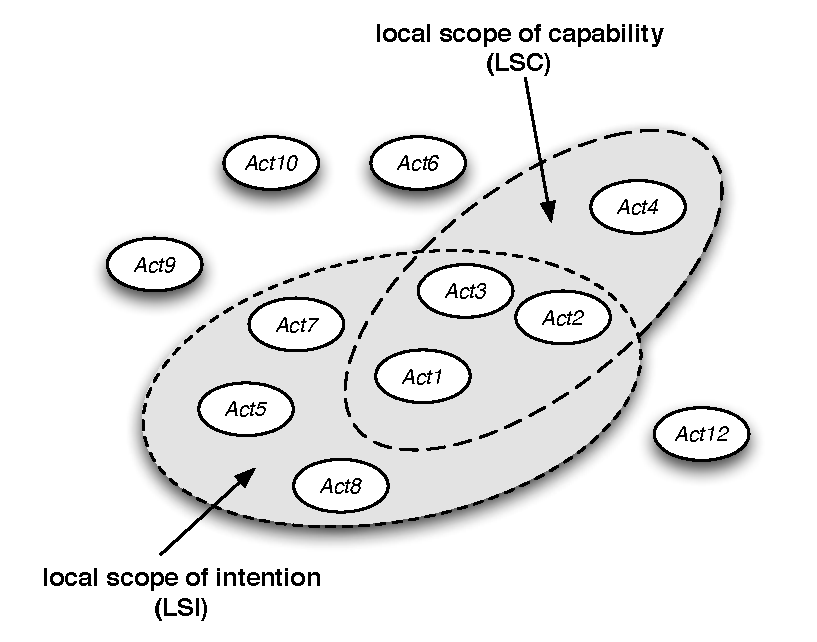
\includegraphics[width=3.5in]{local_scope.pdf} 
   \caption{The structure of local scope of work}
   \label{fig:local_scope}
\end{figure}

One thing to note is that the actions within the same sub-space can have different relations with the actor. That is, the actions in the \emph{local scope of intention} can be either potentially intended ($Pos.Int$), intended that it be performed ($Int.Th$), or intended to be performed ($Int.To$). Similarly, the actions in the \emph{local scope of capability} can also be related to the actor with different levels of capability (i.e. $Knows$, $Able$, $Workable$). As a result, we cannot define the local scope for each actor just as a set of actions, but also with the corresponding relations.

Following this, we define the \emph{local scope of intention} for an actor $LSI(ar)$ as a set of tuples, and each tuple includes three elements: the actor, the action, and the intention relation between them:
\begin{align*} 
	LSI(ar) = \{<ar, act, rel(ar, act)>\}
\end{align*}
where $act\in ACT$ and $rel\in \{Pos.Int, Int.Th, Int.To, Perform\}$.

Similarly, the \emph{local scope of capability} for an actor $LSC(ar)$ is defined as:
\begin{align*} 
	LSC(ar) = \{<ar, act, rel(ar, act)>\}
\end{align*}
where $act\in ACT$ and $rel\in \{Knows, Able, Workable\}$.

Thereafter, the \emph{local scope of work} for an actor $LS(ar)$ is defined as:
\begin{align*} 
	LS(ar) = LSI(ar) \cup LSC(ar)
\end{align*}
% subsection local_scopes (end)
\subsection{Dependencies} % (fold)
\label{sub:dependencies}
We can now focus on the modeling of dependencies between actions. In general, a dependency is defined as a meta-predicate ($DEP$) on two actions ($act_1$, $act_2$) and a proposition $p$, where $act_1$ depends on $act_2$ because of some proposition $p$, and is denoted by $DEP(act_1, act_2, p)$. We follow the terms used in \cite{yu1993actor} to call the depending entity $act_1$ the \emph{depender}, and the entity who is depended upon $act_2$ the \emph{dependee}, and the proposition representing the dependency relation \emph{dependum}.

Based on the various types of relations between actions and resources defined in Section \ref{ssub:relations}, we can use them to define the various types of dependencies described in our conceptual framework in Section \ref{ssub:dependencies}. 

\paragraph*{Temporal dependency} % (fold)
\label{par:temporal_dependencies_}
The predicate $Precedes$ can be used to define the temporal dependency between actions, i.e. the performance of the action $act_2$ as \emph{depender} depends on the performance of the action $act_1$ as \emph{dependee}, because $act_1$ is a pre-requisite action that must have been completed at the time when $a_2$ is performed. $Precedes(act_1, act_2)$ is the \emph{dependum} in this case.
\begin{align*} 
	 DEP(act_2, act_1, Precede(act_1, act_2))
\end{align*}
% paragraph temporal_dependencies_ (end)

\paragraph*{Resource dependencies} % (fold)
\label{par:resource_dependencies}
The predicates $Consumes$ and $Produces$ can be used to define the three types of resource dependencies. 

A \emph{fit dependency} occurs when two actions ($act_1$, $act_2$) collectively produce the same resource ($res_1$). In this case, the two actions  are mutually dependent on each other, i.e. both can be \emph{depender} and \emph{dependee} at the same time. The \emph{dependum} is the combination of two predicates: $Produces(act_1, res_1)$ and $Produces(act_2, res_1)$.
\begin{align*} 
	 DEP(act_1, act_2, Produces(act_1, res_1) \land Produces(act_2, res_1))\\
	 DEP(act_2, act_1, Produces(act_1, res_1) \land Produces(act_2, res_1))
\end{align*}

A \emph{flow dependency} arises whenever one action $act_1$ produces a resource $res_1$ that is used by another action $act_2$, i.e. the performance of the action $act_2$ as \emph{depender} depends on the performance of the action $act_1$ as \emph{dependee}, because of the two predicates: $Produces(act_1, res_1)$ and $Consumes(act_2, res_1)$.
\begin{align*} 
	 DEP(act_2, act_1, Produces(act_1, res_1) \land Consumes(act_2, res_1))
\end{align*}

A \emph{sharing dependency} arises whenever multiple actions both use the same resource. Similar to a fit dependency, the two actions are mutually dependent on each other, because of the two predicates: $Consumes(act_1, res_1)$ and $Consumes(act_2, res_1)$.
\begin{align*} 
	 DEP(act_1, act_2, Consumes(act_1, res_1) \land Consumes(act_2, res_1))\\
	 DEP(act_2, act_1, Consumes(act_1, res_1) \land Consumes(act_2, res_1))
\end{align*}
% paragraph resource_dependencies (end)

\paragraph*{Goal dependency} % (fold)
\label{par:goal_dependency}
The predicate $Sub.Act$ can be used to define the goal decomposition dependency between two actions. It indicates that action $act_2$ depends on action $act_1$ because $act_1$ is a subsidiary action that must have been completed to achieve $act_2$ in current collaborative plan, i.e. $Sub.Act(act_1, act_2)$
\begin{align*} 
	 DEP(act_2, act_1, Sub.Act(act_1, act_2))
\end{align*}
% paragraph goal_dependency (end)
% subsection dependencies (end)
% section formalizaing_the_field_of_work (end)
